% %This is a very basic article template.
% %There is just one section and two subsections.
% \documentclass[a4paper,oneside]{article}
\documentclass[a4paper, 10pt, conference]{ieeeconf} \IEEEoverridecommandlockouts
 % This command is only
  % needed if you want
  % to use the \thanks
  % command
\overrideIEEEmargins
% See the \addtolength command later in the file to balance the column lengths
% on the last page of the document

\usepackage[pdftex, pdftitle={DiagnosabilityVerification of Discrete-Event
Systems}, pdfauthor={Dmitry Myadzelets}, bookmarks=false,
% colorlinks=true, linkcolor=black
]{hyperref}

\usepackage{amsfonts}
\usepackage{graphicx}
\usepackage{epstopdf}
\usepackage{tikz}
\usetikzlibrary{decorations.pathreplacing}
\usetikzlibrary{arrows,positioning,automata,shadows,fit,shapes}

% \usepackage{fancyheadings} \pagestyle{fancyplain}
% \lhead[\fancyplain{}{}]{\fancyplain{}{DRAFT}}
% \rhead[\fancyplain{}{}]{\fancyplain{}{\today}}

\begin{document}

\title{Non-Compositional Analysis of Discrete-Event Systems \\
with Modular Structure}
\author{Draft \\ \today}
% \author{Dmitry Myadzelets$^{*,1,2}$, Andrea Paoli$^{1,3}$%, \today
% \thanks{$^{1}$Center for Research on Complex Automated Systems (CASY), DEI,
% University of Bologna, Viale Pepoli 3/2, 40123, Bologna, Italy}
% 	\thanks{$^{2}$E-mail: {dmitrymyadzelets@gmail.com}}
% 	\thanks{$^{3}$E-mail: {andrea.paoli@unibo.it}} 
% } 
\maketitle

% To meet requirements of EU funding
% http://eacea.ec.europa.eu/about/eacea_logos_en.php "This project has been
% funded with support from the European Commission. This publication reflects
% the views only of the author, and the Commission cannot be held responsible
% for any use which may be made of the information contained therein."
% \begin{figure}[!b]
% \begin{tabular}{l p{60mm}} 
%  	\includegraphics[height=10mm]{EU_flag.eps}
%  	& \vspace{-10mm} \footnotesize
%  	$^{*}$With the support of the Erasmus Mundus Action 2 programme of the
%  	European Union. 
% \end{tabular}
% \end{figure}

\begin{abstract}
This paper describes methods of analysing the structure of modules of
discrete-event systems in order to verify their diagnosability property.
The methods imply that no parallel composition of the modules needs to be
performed, thus reducing complexity of the analysis of the property. The methods
may be considered as preliminary steps for other techniques, or used to find a
guiding criteria in the methods performing iterative composition of the modules.
An example of the approach is included.
\end{abstract}

\newtheorem{assumption}{Assumption}
\newtheorem{definition}{Definition}
\newtheorem{conjecture}{Conjecture}
\newtheorem{corollary}{Corollary}
\newtheorem{example}{Example}
\newtheorem{theorem}{Theorem}

% %%%%%%%%%%%%%%%%%%%%%%%%%%%%%%%%%%%%%%%%%%%%%%%%%%%%%%%%%%%%%%%%%%%%%%%%%%%%%%
\section{Introduction}
% Ruffly: What we are talking about and what problem exist there in general. How
% the problems are solved. What we suggest exactly and what is that for.
% How this paper is structured.
Discrete-Event Systems (DES) has successfully concurred significant area in
systems engineering discipline due to their enormous capabilities of designing
and managing complex projects. While ``real-world'' systems are growing in scale
the solutions DES provide have to evolve in order to tackle increasing
complexity issues. Development of solutions relying on the fact that the most of
complex system have naturally modular structure thus has been under focus for
the last two decades. Particularly, the task of design verification and
diagnosis with respect to undesired behaviour, commonly refereed as to faulty
behaviour, of discrete systems has a fairly developed theory nowadays.

The most of approaches for diagnosability verification of modular discrete
systems involve parallel composition of the modules. Consequently, these
solutions suffer from exponential complexity. However, its unlikely
that computational expenses for a model of ``real-world'' system reach its
theoretical upper bound. Thus there is still a room for the techniques aimed to
improve design verification of modular discrete-event systems by decreasing
resources required for that.

This paper consider evaluation of modules' structure with respect to
diagnosability property in order to find logical conditions of the system either
be diagnosable or not diagnosable, without parallel composition of the modules.
In this paper a general DES with modular structure is assumed, and that each
module of the system has a corresponded predefined model.
We exploit the automata framework for the model representation, i.e. we assume
that each module of the system is represented by a regular language and a
correspondent automaton.

This paper is organized as follows. Section \ref{sec:Preliminaries} covers the
necessary notation and describes the diagnosability problem. Section
\ref{sec:Proposal} focuses on analysis of a module when it models both
non-faulty and faulty behaviour. Section \ref{sec:} analyses structure of
modules which have events common with the module a faulty behaviour originates
from. The last Section \ref{sec:Conclusion} concludes current results and
discuss possible directions for further research.

% %%%%%%%%%%%%%%%%%%%%%%%%%%%%%%%%%%%%%%%%%%%%%%%%%%%%%%%%%%%%%%%%%%%%%%%%%%%%%%
% \subsection{Heuristic}
% \label{sec:heuristic}
% The known approaches for diagnosability analysis assume that the number of
% diagnosers is defined at the input[proof?], and the order the modules of the
% system are composed during iterations is not considered. However, our heuristic
% is following:
% \begin{enumerate}
%   \item The number of diagnosers can be optimised in order to reduce
%   communications among them;
%   \item The order of composition can be tuned to archive lower computational
%   expenses.
% \end{enumerate}
% 
% The heuristic is based on the observations:
% \begin{enumerate}
%   \item We know for all the components if each of them has events in common with
%   any other component, i.e. if any two components are coupled by the common
%   events.
%   \item The coupling has its own \emph{properties} both quantitative and
%   qualitative, as a number of the common events, presence of string with only one common event,
%   number of transitions between two common events in strings, and etc.
%   \item For any given model of a component in the system exists a
%   diagnoser, or we know what diagnosability property it has.
%   \item The diagnosability property can be either changed or not if the module
%   is composed with other modules coupled with it. 
%   We may say that coupling can change the diagnosability property of each module
%   involved.
%   \item In order to verify (some) diagnosability properties of the system we
%   have to compose all the components which affect these properties.
%   \item Thus, based on the coupling properties we can guide the
%   iterative compositional process. The most intuitive aim for the guidance is
%   computational expense.
%   \item In a target system either the components or their diagnosers might be
%   grouped in order to decrease modularity. The resulting components have their
%   own coupling properties. These properties have a relation to a
%   necessary communication among modules during the on-line diagnosis.
%   \item The coupling properties can be changed by manipulating of the grouping,
%   thus, changing the communication load, even down to zero.
% \end{enumerate}

% \begin{enumerate}
%   \item Algorithm to compose and create macro modules.
%   \item Method to check distributed diagnosability without a
%   central decision point and communication protocol.
% \end{enumerate}
% Criteria of the coupling could be aimed for minimal time or/and space expenses. 


%%%%%%%%%%%%%%%%%%%%%%%%%%%%%%%%%%%%%%%%%%%%%%%%%%%%%%%%%%%%%%%%%%%%%%%%%%%%%%%
\section{Preliminaries}
\label{sec:Preliminaries}
The notation used in this document is adopted from
\cite{cassandras_introduction_2010}.

Let $\Sigma$ be a finite set of events. An sequence of events is a string.
$\Sigma^*$ denotes a set of finite strings over $\Sigma$. $L\subseteq\Sigma^*$
is a language over $\Sigma$. Given strings $s$ and $t$, $st$ is their
concatenation. Given strings $s$ and $s'$, $s'$ is a prefix of $s$ if exists $t$
such that $s't = s$. Prefix closer of $L$, denoted by $\overline{L}$ is a set of
all prefixes of all strings in $L$.
If $\overline{L} = L$ then $L$ is prefix-closed. The post language of $L$ after
a string $s$ is denoted as $L/s$, i.e. $L/s = \{t\mid st \in L\}$.

An automaton $G$ is a tuple $$G=(X,\Sigma,\Delta,x_0, X_m),$$ where $X$ is a
set of states, $x_0 \in X$ is an initial state, $X_m \subseteq X$ is the set of
marked states, and $\Delta: X \times \Sigma \rightarrow X$ is the transition
function.
We say the a language $L$ is generated or recognized by the automaton $G$, $L =
\mathcal{L}(G)$. In this paper we assume that for each language there is always
a correspondent automaton, and vice versa. The marked language $L_m \subseteq
L$ is intended to make a part of the automaton's behaviour distinguishable.

Some events of DES might not be observed. To reflect that the set of events
$\Sigma$ is partitioned into disjointed sets of observable events $\Sigma_o$ and
not observable events $\Sigma_{ou}$ such that $\Sigma = \Sigma_o~\dot{\cup}~
\Sigma_{ou}$.
The $M: \Sigma^* \rightarrow \Sigma_o^*$ denotes the natural projection that
erases unobservable events, where $\epsilon$ means the empty string. The
correspondent inverse projection is $M^{-1}: \Sigma_o \rightarrow 2^\Sigma$. If
a set of observable events is partitioned into subsets, such that $\Sigma_o =
\bigcup_i \Sigma_{i,o} \mid i \in \mathbb{N}$, the natural projection over the
partition members is denoted as $M_i: \Sigma^* \rightarrow \Sigma_{i,o}^*$.

% \subsection{Review of existing approaches for diagnosability}
% \begin{enumerate}
%   \item Construction of a complex system $G = \parallel G_i$, and building a
%   diagnoser $D$ for the system; 
%   \item Construction of a complex system $G = \parallel G_i$, and building a set
%   of diagnosers $\{D_i \ldots D_n\}$ with a central decision node;
%   \item Construction of a complex system $G = \parallel G_i$, and building a set
%   of diagnosers $\{D_i \ldots D_n\}$ where the diagnosers communicate to each
%   other;
%   \item Modular diagnosability.
% \end{enumerate}
% 
% In \cite{garcia_centralized_2002} the authors study a modular
% decomposition, and provide a method to avoid coupling of diagnosers.
% (Andrea referenced to that work in one of his paper \cite{paoli_safe_2003}).

% \subsubsection{Modular Diagnosability}
% \label{sec:modular_diagnosability}
% A notion of modular diagnosability is introduced in
% \cite{contant_diagnosability_2006}. The authors define it as the ability to
% diagnose a system on-line using only local diagnosers with no communications
% among them. The paper presents a verification algorithm to check if the system
% is modular diagnosable. It worth noting that the local diagnosers might be
% modified during verification process.
% 
% \paragraph{Assumptions} in the paper are following:
% \begin{enumerate}
%   \item Common events are observable;
%   \item Faults are local;
%   \item At least one observable event in each indeterminate cycle;
%   \item The language of the system is live (the authors note this can be
%   relaxed).
% \end{enumerate}
% 
% \paragraph{The algorithm} for verification of modular diagnosability works like
% that. Check if all the modules are locally diagnosable. If so then the system is
% modular diagnosable. Otherwise for each non-diagnosable modules do next: extract
% the indeterminate cycle and construct the observer (deterministic projection) of
% the common events; make parallel composition of the projection with similar
% projections of other modules with common events (keep the sets of the
% modules' common events, not the diagnosers); 
% check diagnosability, and so on.
% 
% \paragraph{Our notes}
% \begin{enumerate}
%   \item To verify diagnosability property of a module it seems possible to use,
%   instead of a diagnoser, the verifier \cite{yoo_polynomial-time_2002} or the
%   partitioning to faulty and non-faulty languages with consequent parallel
%   composition with respect to observable events \cite{cassez_note_2009}.
%   \item If a module is diagnosable, the property can be changed after the
%   composition, can't be it?
%   \item Complexity of the approach is not presented, but it seems to
%   be exponential due to the construction of diagnosers and parallel composition
%   of them.
% \end{enumerate}


%%%%%%%%%%%%%%%%%%%%%%%%%%%%%%%%%%%%%%%%%%%%%%%%%%%%%%%%%%%%%%%%%%%%%%%%%%%%%%%
A system is defined by a set of automata $\{G_{i \in \mathbb{N}}\}$ and a
corresponded set of languages $\{L_{i \in \mathbb{N}}\}$. We use the term
\emph{local} in context of the automata and languages from these sets. The
\emph{global} language of the system is thus defined by the parallel
composition of its local languages: $L = \parallel_{i \in \mathbb{N}} L_i$.

\subsection{Synchronized (coupled) languages}
Given sets of events $\Sigma = \Sigma_1 \cup \Sigma_2$, and
two languages $L_1 \subseteq \Sigma_1^*$ and $L_2 \subseteq \Sigma_2^*$.
If $\Sigma_1 \cap \Sigma_2 \neq \emptyset$ then we say that the languages $L_1$ and
$L_2$ are coupled (synchronised). The subset of $L_1$, the all strings which
have common events in it, is defined as:
\begin{equation}
\label{eq_synchronized_language}
L'_{1} =
	L_1 \cap \left( \Sigma_1^* \{\sigma\} \Sigma^* \right) 
	\mid \sigma \in \Sigma_1 \cap \Sigma_2.
\end{equation}
By the definition $L'_1 \subseteq L_1$ and, in general, it is not
prefix-closed, $L'_1 \subseteq \overline{L'_1}$.

\subsection{Projections} On events:
\label{sec:projections}
$$P_{i,j} : \Sigma_i \rightarrow \Sigma_i \cap \Sigma_j,$$
and its version for the languages: 
$$P_{i,j} : L_i \rightarrow (\Sigma_i \cap \Sigma_j)^*.$$

Inverse projections: (skipped). 
The language $L'_1$ can equally be defined with the inverse projection:
$$
L'_1 = P^{-1}_{1,2}(\Sigma_1 \cap \Sigma_2)^*.
$$

% \subsubsection{Quantified properties} The language $L_i \backslash L'_i$ has
% no common events. The size of the language $n = |L_i \backslash L'_i|$ and the
% size of the adjacent language $m = |L_j \backslash L'_j|$ allows us to
% calculate the size of their parallel composition a priori, i.e.
% $|L'_i \parallel L'_j| = m \times n$.
% Non-deadlocking sub-language:
% $$
% L''_i \subseteq L_i \mid \forall s \in L''_i, |P_i(s)| \leq 1 
% $$
% is the language which has string with no common events or with only one common
% event. This language being composed with an adjacent one never leads to
% deadlocks. Then, the sub-language $L_i \cap L''_i$ is potentially deadlocking.
% The size of the language after the parallel composition for non-deadlocking
% sub-languages is also can be calculated a priori (what is complexity of that?).
% 
% If a module has only non-deadlocking language, the module can be skipped in the
% process of the liveness verification, and it does not affect diagnosability
% property as well.
% 
% The size of the resulting composition with respect to the language $L_i
% \backslash L''_i$ seems hardly computable for a large system, however the size
% of it in the worse case is known.


%%%%%%%%%%%%%%%%%%%%%%%%%%%%%%%%%%%%%%%%%%%%%%%%%%%%%%%%%%%%%%%%%%%%%%%%%%%%%%%
\section{Diagnosability of a modular system}
\label{sec:Diagnosability}
%\subsection{Faulty and non-faulty languages}
Diagnosability analysis uses the notion of a faulty language to describe a
faulty behaviour of discrete-event system. This section focuses on the
design issues relates to representation of the faulty language.  

A faulty behavior is usually modeled by introducing fault events or by faulty
and non-faulty specifications. The approaches are also known as
\emph{event-based} and \emph{state-based} correspondingly. 

In the event-based approach fault events are a special type of event, such
that $\Sigma$ can be disjointed into the sets of faults $\Sigma_f$ and
non-faults $\Sigma\backslash \Sigma_f$. A string containing a fault event is
called \emph{faulty string}, i.e. $s \in \Sigma^*\Sigma_f\Sigma^*$. A set of faulty
strings is called \emph{faulty language}, i.e. formally $$L_f = \{ s \in
\Sigma^*\Sigma_f\Sigma^* \} \mid s \in L.$$
By definition, the faulty language is not prefix-closed in general, $L_f
\subseteq L$. The \emph{non-faulty language} is defined here as $L_{nf} = L
\backslash L_f$.
If the faulty behaviour defined by the event-based approach the language of the
system can be partitioned into faulty and non-faulty sub-languages. An example
of automata reflecting the partitioning of a language is depicted in Figure
\ref{fig_automaton_F-NF}.

% To distinguish strings ending with fault events and containing fault events we
% define the \emph{strictly faulty language}
% $$L_f^= = \{s \in \Sigma^*\Sigma_f\}.$$ 

In the case of the state-based approach the faulty specification
allows us to define undesired behavior when fault events are
not necessarily introduced. Since the the faulty language is not prefix-closed
in general, the marked language is used to distinguish it from non-faulty
language.

% To unify both approaches, we define the strictly-faulty language in the
% later case as $$L_f^= = \{s\sigma \in L_f | s \not \in L_f, \sigma \in \Sigma
% \},$$ and fault occurrence implies that an event of a string $s \in L_f^=$
% occurs.

For the sake of clarity we introduce a generalized schema of the
partitioning, as it is depicted in Figure \ref{fig_partitioning_faulty}. The
schema shows a general structure of a language with a faulty behaviour defined
by both approaches. There $f$-point express either a set of fault events or
states after which the language considered as faulty.  

Different undesired behaviours are defined by partitioning $\Sigma_f$ into
subsets (not necessarily disjoint) or by several specifications. For the sake of
brevity we refer to each undesired behaviour as to one fault type or simpy
fault.

We define \emph{diagnosability of a fault} as follows:
\begin{definition} The fault is \emph{not diagnosable} if there are two strings
with same observation such that one string is faulty and of infinite length, and
second one is no faulty, i.e.
 $$
	(\exists s \in L_f, t \in L_{nf})(|s| = \infty)(M(s) = M(t)).
$$ 
Consequently, the fault is \emph{diagnosable} if there is no such strings.
\end{definition}
We define \emph{diagnosability of the language} as follows:
\begin{definition}
The language is diagnosable if its all faults are diagnosable.
\end{definition}

In the above the infinite length of the string $s$ is equal to the statement
that the string $s$ forms a cycle. This definition is more weak then one
presented in \cite{sampath_diagnosability_1995} because it does not assume non
existence of unobservable cycles.
   
\begin{figure}[t]
\centering
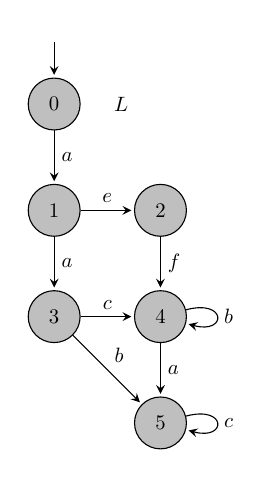
\begin{tikzpicture} 
[->,>=stealth, node distance=18mm, auto, initial text=, on grid,
shorten >=1pt, every state/.style={fill=lightgray}, 
every node/.style={scale=0.75}, 
accepting/.style={double distance=1.5pt, outer sep=0.75pt+\pgflinewidth}] 
	\node[state, initial above]	(0) 					{$0$};
	\node[state]			(1) [below of = 0]		{$1$};
	\node[state]			(2) [right of = 1]		{$2$};
	\node[state]			(3) [below of = 1]		{$3$};
	\node[state]			(4) [right of = 3]		{$4$};
	\node[state]			(5) [below of = 4]		{$5$};
	\node[right of = 0] at (-.5,0) {$L$};
		
  	\path
  		(0) edge 				node {$a$} (1)
  		(1) edge 				node {$e$} (2)
  		(1) edge 				node {$a$} (3)
  		(2) edge 				node {$f$} (4)
  		(3) edge 				node {$c$} (4)
  		(3) edge 				node {$b$} (5)
  		(4) edge [loop right]	node {$b$} (4)
  		(4) edge 				node {$a$} (5)
  		(5) edge [loop right]	node {$c$} (5);
\end{tikzpicture}
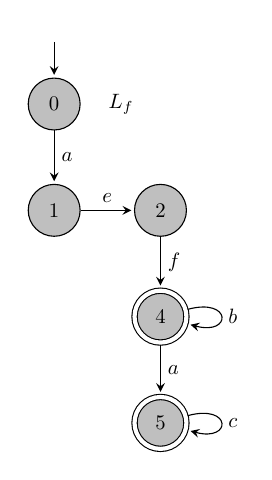
\begin{tikzpicture}
[->,>=stealth, node distance=18mm, auto, initial text=, on grid, shorten >=1pt,
every state/.style={fill=lightgray},
every node/.style={scale=0.75},
accepting/.style={double distance=1.5pt, outer sep=0.75pt+\pgflinewidth}
]
	\node[state, initial above]	(0) 					{$0$};
	\node[state]			(1) [below of = 0]		{$1$};
	\node[state]			(2) [right of = 1]		{$2$};
	\node[state, accepting]	(4) [below of = 2]		{$4$};
	\node[state, accepting]	(5) [below of = 4]		{$5$};
	\node[right of = 0] at (-.5,0) {$L_f$};
	
  	\path
  		(0) edge 				node {$a$} (1)
  		(1) edge 				node {$e$} (2)
  		(2) edge 				node {$f$} (4)
  		(4) edge [loop right]	node {$b$} (4)
  		(4) edge 				node {$a$} (5)
  		(5) edge [loop right]	node {$c$} (5);
\end{tikzpicture}
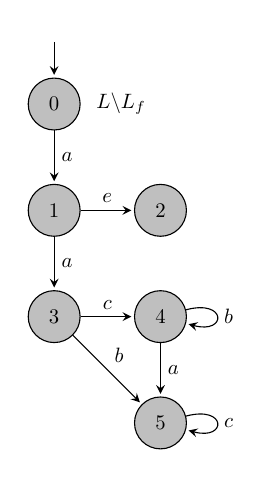
\begin{tikzpicture}
[->,>=stealth, node distance=18mm, auto, initial text=, on grid, shorten >=1pt,
every state/.style={fill=lightgray}, 
every node/.style={scale=0.75},
accepting/.style={double distance=1.5pt, outer sep=0.75pt+\pgflinewidth}
]
	\node[state, initial above]	(0) 					{$0$};
	\node[state]			(1) [below of = 0]		{$1$};
	\node[state]			(2) [right of = 1]		{$2$};
	\node[state]			(3) [below of = 1]		{$3$};
	\node[state]			(4) [right of = 3]		{$4$};
	\node[state]			(5) [below of = 4]		{$5$};
	\node[right of = 0] at (-.5,0) {$L\backslash L_f$};
	
  	\path
  		(0) edge 				node {$a$} (1)
  		(1) edge 				node {$e$} (2)
  		(1) edge 				node {$a$} (3)
  		(3) edge 				node {$c$} (4)
  		(3) edge 				node {$b$} (5)
  		(4) edge [loop right]	node {$b$} (4)
  		(4) edge 				node {$a$} (5)
  		(5) edge [loop right]	node {$c$} (5);
\end{tikzpicture}
\caption{Automata representing a language $L$, faulty language $L_f$ and
non-faulty language $L \backslash L_f$, given $\Sigma_f = \{f\}$}
\label{fig_automaton_F-NF}
\end{figure}

\begin{figure}[t]
\centering
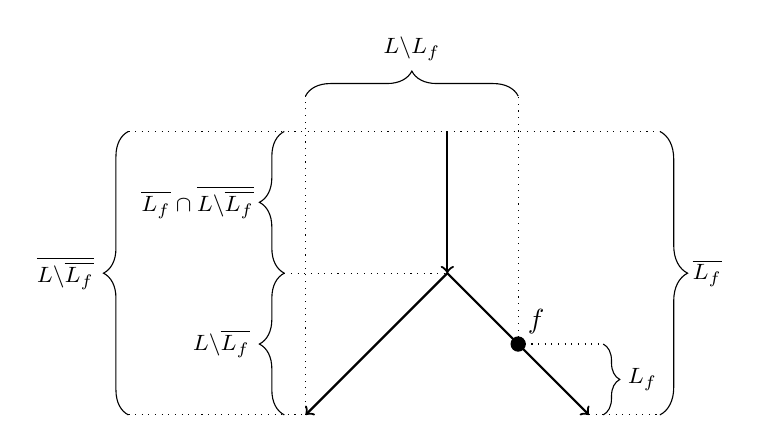
\begin{tikzpicture}[scale=.9]
% Y
\draw [thick] [->](4,5)--(4,3);
\draw [thick] [->](4,3)--(6,1);
\draw [thick] [->](4,3)--(2,1);
% Events
\draw [fill] (5,2) circle [radius=0.1];
\node [above right] at (5,2) {$f$};
% Braces
\draw [decorate,decoration={brace,amplitude=10pt}]
 	(7,5)--(7,1) node [midway,xshift=0.6cm] {\footnotesize $\overline{L_f}$};
\draw [decorate,decoration={brace,amplitude=6pt},xshift=2mm]
 	(6,2)--(6,1) node [midway,xshift=0.5cm] {\footnotesize $L_f$};
\draw [decorate,decoration={brace,amplitude=9pt}]
 	(2,5.5)--(5,5.5) node [midway,yshift=0.6cm] {\footnotesize $L\backslash
 	L_{f}$};
\draw [decorate,decoration={brace,amplitude=9pt},xshift=-3mm]
  	(2,1)--(2,3) node [midway,xshift=-8mm] {\footnotesize $L\backslash
  	\overline{L_{f}}$};
\draw [decorate,decoration={brace,amplitude=9pt},xshift=-3mm]
 	(2,3)--(2,5) node [midway,xshift=-11mm] {\footnotesize $\overline{L_f} \cap
  	\overline{L\backslash \overline{L_{f}}}$};
\draw [decorate,decoration={brace,amplitude=9pt},xshift=-5mm]
  	(0,1)--(0,5) node [midway,xshift=-8mm] 
  	{\footnotesize $\overline{L\backslash \overline{L_{f}}}$};
%Dashed lines
\draw [dotted] (5,2)--(5,5.5);
\draw [dotted] (2,1)--(2,5.5);
\draw [dotted] (6,1)--(7,1);
\draw [dotted] (5,2)--(6.2,2); 
\draw [dotted] (-0.5,5)--(7,5);
\draw [dotted] (-0.5,1)--(2,1);
\draw [dotted] (1.7,3)--(4,3);
% % Y
% \draw [thick] [->](4,2)--(4,4);
% \draw [thick] [->](4,4)--(2,6);
% \draw [thick] [->](4,4)--(6,6);
% % Events
% \draw [fill] (3,5) circle [radius=0.1];
% \node [above right] at (3,5) {$f$};
% % Braces
% \draw [decorate,decoration={brace,amplitude=10pt}]
%  	(1,2)--(1,6) node [midway,xshift=-0.6cm] {\footnotesize $\overline{L_f}$};
% \draw [decorate,decoration={brace,amplitude=6pt},xshift=-6pt]
%  	(2,5)--(2,6) node [midway,xshift=-0.6cm] {\footnotesize $L_f$};
% \draw [decorate,decoration={brace,amplitude=9pt}]
%  	(6,1)--(3,1) node [midway,yshift=-0.6cm] {\footnotesize $L\backslash L_{f}$};
% \draw [decorate,decoration={brace,amplitude=9pt},xshift=0.3cm]
%  	(6,6)--(6,4) node [midway,xshift=.8cm] {\footnotesize $L\backslash
%  	\overline{L_{f}}$};
% \draw [decorate,decoration={brace,amplitude=9pt},xshift=0.3cm]
%  	(6,4)--(6,2) node [midway,xshift=1.1cm] {\footnotesize $\overline{L_f} \cap
%  	\overline{L\backslash \overline{L_{f}}}$};
% \draw [decorate,decoration={brace,amplitude=9pt},xshift=.5cm]
%  	(7.6,6)--(7.6,2) node [midway,xshift=.8cm] 
%  	{\footnotesize $\overline{L\backslash \overline{L_{f}}}$};
% %Dashed lines
% \draw [dotted] (1,6)--(2,6);
% \draw [dotted] (1,2)--(8.1,2);
% \draw [dotted] (1.8,5)--(3,5); 
% \draw [dotted] (3,1)--(3,5);
% \draw [dotted] (6,1)--(6,6);
% \draw [dotted] (6,6)--(8.1,6);
% \draw [dotted] (4,4)--(6.3,4);

% Language L_V
% \draw [thick] [->](9,5)--(9,1);
% \draw [fill] (9,2) circle [radius=0.1];
% \node [left] at (9,2) {$f$};
% \draw [decorate,decoration={brace,amplitude=6pt},xshift=0.6cm]
%  	(9,2)--(9,1) node [midway,xshift=0.6cm] {\footnotesize $L_{V,f}$};
% \draw [decorate,decoration={brace,amplitude=9pt},xshift=0.6cm]
%  	(9,5)--(9,2) node [midway,xshift=1cm] {\footnotesize
%  	$L_V\backslash L_{V,f}$};
% \draw [dotted] (9,5)--(9.6,5);
% \draw [dotted] (9,2)--(9.6,2);
% \draw [dotted] (9,1)--(9.6,1);
\end{tikzpicture}
\caption{Structural schema of a language $L$ partitioned into the faulty
language $L_f$ and non-faulty language $L \backslash L_f$}
\label{fig_partitioning_faulty}
\end{figure}

In this paper we assume that faulty and non-faulty languages are known for the
modules of the system. We also assume for the sake of simplicity that there is
only one type of fault, such that it is not necessary to identify
which type of fault occurred.

\subsection{Architectures for on-line diagnosis}
In the following we present a general classification of the
architectures for on-line diagnosis presented in literature. They may be divided
in three types: centralized, decentralized and distributed. 
% The most of
% approaches exploits a diagnoser \cite{sampath_diagnosability_1995} for on-line
% diagnosis

\subsubsection{Centralized}
The structure of the centralized diagnosis is depicted in 
Figure \ref{fig_centralized}. In this architecture the global language is
built by the parallel composition and then the diagnoser $D$ introduced in
\cite{sampath_diagnosability_1995} for the global language is constructed. Upon
the current state of the diagnoser a decision on the fault occurrence is made.

\begin{figure}[t]
\centering
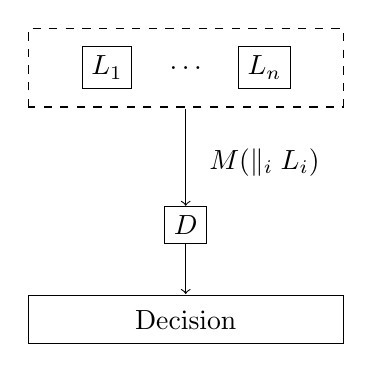
\begin{tikzpicture}
	\node[draw]		(0)	at (1, 3) 		{$L_1$};
	\node[]			(1)	[right of = 0]	{$\ldots$};
	\node[draw]		(2)	[right of = 1]	{$L_n$};
	\draw[dashed] (0, 2.5) rectangle (4, 3.5);
	\node[]			(3) at (2, 2.6) {};
	\node[draw]		(4) at (2, 1) {$D$};	
	\draw[->] (3) -- (4);
	\node[]	at (3, 1.8) {$M(\parallel_{i} L_i)$};
	\node[]		(5) [below of = 4] {};	
	\draw[->] (4) -- (5);
	\draw[] (0, -.5) rectangle (4, 0.1);
	\node[]			(3) at (2, -.2) {Decision};
	
\end{tikzpicture}
\caption{Architecture of a system with centralized diagnosis}
\label{fig_centralized}
\end{figure}

\subsubsection{Decentralized}
In the approach only local diagnosers are built.
The diagnosers provide a necessary information (a protocol) to a central
decision node. The diagnosers do not communicate to each other. This
architecture is depicted in Figure \ref{fig_decentralized}.
Notable works on decentralized architecture are
\cite{debouk_coordinated_1998},
\cite{contant_diagnosability_2006} and \cite{wang_diagnosis_2007}.

\begin{figure}[t]
\centering
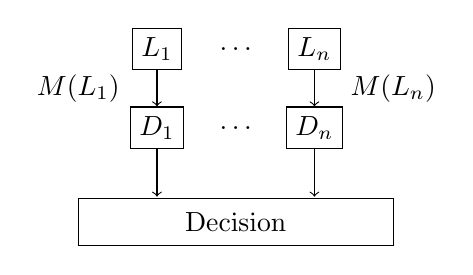
\begin{tikzpicture}
	\node[draw]		(0)	at (1, 2) 		{$L_1$};
	\node[draw]		(00) [below of = 0] {$D_1$};
	\node[]			(10) [below of = 00] {$$};
	\draw[->] (0) -- (00);
	\draw[->] (00) -- (10);
	
	\node[]			(1)	[right of = 0]	{$\ldots$};
	\node[]			(11)[right of = 00]	{$\ldots$};
	
	\node[draw]		(2)	[right of = 1]	{$L_n$};
	\node[draw]		(22) [below of = 2] {$D_n$};
	\node[]			(20) [below of = 22] {$$};
	\draw[->] (2) -- (22);
	\draw[->] (22) -- (20);

	\node[]	at (0, 1.5) {$M(L_1)$};
	\node[]	at (4, 1.5) {$M(L_n)$};
	
	\draw[] (0, -.5) rectangle (4, 0.1);
	\node[]			(3) at (2, -.2) {Decision};
\end{tikzpicture}
\caption{Architecture of a system with decentralized diagnosis}
\label{fig_decentralized}
\end{figure}

\subsubsection{Distributed}
The architecture is depicted in Figure \ref{fig_distributed}. 
An example of the approach can be found in \cite{pencole_formal_2005} and
\cite{schumann_decentralised_2010}.

\begin{figure}[t] 
\centering
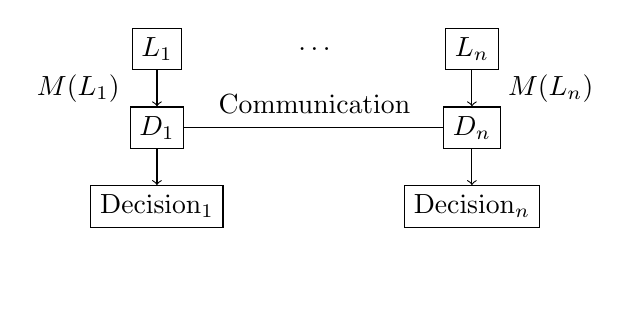
\begin{tikzpicture}
	\node[draw]		(0)	at (1, 2) 		{$L_1$};
	\node[draw]		(00) [below of = 0] {$D_1$};
	\node[draw]		(p0) [below of = 00] {Decision$_1$};
	\node[]			(10) [below of = p0] {$$};
	\draw[->] (0) -- (00);
	\draw[->] (00) -- (p0);
	
	\node[]			(1)	at (3, 2)	{$\ldots$};
	\node[] at (3, 1.3) {Communication};
	
	\node[draw]		(2)	at (5, 2) 		{$L_n$};
	\node[draw]		(22) [below of = 2] {$D_n$};
	\node[draw]		(p2) [below of = 22] {Decision$_n$};
	\node[]			(20) [below of = 22] {$$};
	\draw[->] (2) -- (22);
	\draw[->] (22) -- (p2);
	\draw[] (00) -- (22);

	\node[]	at (0, 1.5) {$M(L_1)$};
	\node[]	at (6, 1.5) {$M(L_n)$};
\end{tikzpicture}
\caption{Architecture of a system with distributed diagnosis}
\label{fig_distributed}
\end{figure}

As it was stated in the section \ref{sec:heuristic} one of the our heuristic is
that we can can tune the order the components are composed to lower the
computational expenses. During an iterative process of the composition the
following questions should be answered:
\begin{enumerate}
  \item Is there a way to analyse the system with respect to diagnosability with
  no composition involved (non-compositional analysis)?
  \item Given a non-diagnosable module and an adjacent one, should we take
  the last one as a candidate for the composition?
  \item If we have two modules can be taken which might be preferred to be
  composed first?
\end{enumerate}

Answers are given in the sequel.

\section{Non-compositional analysis}
\label{sec:Proposal}
Non-compositional analysis should be the fist necessary step
to decide whether the system is not-diagnosable, before we start potentially more
computationally expensive compositional analysis. This step can be found in
some works but it is not considered as a separate topic there. A couple of works
is reviewed further.

In the work \cite{debouk_modular_2002} the authors study modular approach
aimed to decide in an incremental fashion if a global system is diagnosable. In
the Theorem 3.1 they state that the system is diagnosable if each module is
diagnosable. In the authors' verification algorithm the first step may be
referred as to the non-compositional analysis. The step can be describe as
follows: for each module check if it has indeterminate cycle in its diagnoser.
If there is no such cycle then the system is diagnosable. 

The non-compositional analysis equal to the above is presented in the work
\cite{contant_diagnosability_2006}. The authors study modular diagnosability,
and criteria for the system to be non-diagnosable is the existence of
an indeterminate cycle. They establish the following results: 
``(a) if an indeterminate cycle exists in the monolithic diagnoser then
necessarily one of the local diagnosers contains an indeterminate cycle; 
(b) if none of the local diagnosers contains an indeterminate cycle then the
monolithic diagnoser does not contain an indeterminate cycle; and 
(c) if an indeterminate cycle exists in a local diagnoser then it may or may not
exist in the monolithic diagnoser''.
The cases (a) and (b) can be referred as to the non-compositional analysis, and
the correspondent step of checking each module for an indeterminate
cycle in its diagnoser is provided by the authors in the Algorithm 1.

It can be seen from the above, that the non-compositional analysis has
been limited only for checking of indeterminate cycle. In the following we
extend the non-compositional analysis and provide additional conditions for
diagnosability. Firstly we consider analysis of a module the faulty
behavior originates from, then we consider analysis of its adjacent modules.  


%%%%%%%%%%%%%%%%%%%%%%%%%%%%%%%%%%%%%%%%%%%%%%%%%%%%%%%%%%%%%%%%%%%%%%%%%%%%%%%
\subsection{Analysis of a module with a faulty behaviour}
In this section we define sufficient and necessary conditions for diagnosability
by analysing only the module with a faulty behaviour.

Given a system $G$ with two modules $\{G_1, G_2\}$ and
their languages $\{L_1, L_2\}$. The language of the system is $L = L_1 \parallel
L_2$. 
The language of each module is partitioned into faulty $L_{i,f}\mid i\in
\{1,2\}$ and non-faulty $L_i\backslash L_{i,f}$ languages.

In cases when definition of diagnosability does not require any bounds for
faults to be detected, the sufficient condition for diagnosability is the
condition when no indeterminate cycle exists in any module. 
It is expressed in the following theorem (adopted from the aforementioned works)
under assumption that the languages are live:
\begin{theorem}[Sufficient condition for diagnosability]
\label{trm_sufficient_for_diag}
\begin{equation}
\begin{array}{l}
	L \textrm{ is }D \Rightarrow 
	\\[1ex]
	\forall i \in |\{L_i\}|
	\\[1ex]
	\textrm{there is no indeterminate cycle in } Diag(L_i)
\end{array}
\end{equation}
\end{theorem}

% \begin{conjecture}[Sufficient condition for non-diagnosability]
% If $\overline{L_{i,f}}$ has neither observable nor common events, then the
%   system is not diagnosable, i.e:
% \begin{equation}
% \begin{array}{l}
% 	(\forall s \in \overline{L_{i,f}}) 
% 	(P_{i,j}(s) = \epsilon \land \textrm{ and }
% 	M(s) = \epsilon) \Rightarrow L \textrm{ not }D,
% 	\\[1ex] 
% 	or, equally:
% 	\\[1ex]
% 	P_{i,j}(\overline{L_{i,f}}) = \emptyset \textrm{ and }
% 	M(\overline{L_{i,f}}) = \emptyset \Rightarrow L \textrm{ not }D.
% \end{array}
% \end{equation}
% \end{conjecture}
% 
% \begin{corollary}[Necessary condition for diagnosability] The system is
% diagnosable only if at least one string in $\overline{L_{i,f}}$ has common or
% observable events, i.e:
% \begin{equation}
% \begin{array}{l}
% 	L \textrm{ is }D \Rightarrow \exists s \in \overline{L_{i,f}} \mid 
% 	P_{i,j}(s) \neq \epsilon \textrm{ or } M(s) \neq \epsilon,
% 	\\[1ex]
%  	or, equally:
% 	\\[1ex]
% 	L \textrm{ is }D \Rightarrow
% 	P_{i,j}(\overline{L_{i,f}}) \neq \emptyset \textrm{ or }
% 	M(\overline{L_{i,f}}) \neq \emptyset 
% \end{array}
% \end{equation}
% \end{corollary}

% (this condition implies the former conjecture, so no need for the above one)

We augment the above sufficient condition for diagnosability by a sufficient
condition for non-diagnosability and the following necessary condition for
diagnosability.
 \begin{conjecture}[Sufficient condition for non-diagnosability]
If $\exists s \in L_f$ which has no observable events, and $\overline{s}$ has no
common events, then the system is not diagnosable, i.e:
\begin{equation}
\begin{array}{l}
	(\exists s \in L_{i,f}) 
	\left[
		P_{i,j}(\overline{s}) = \epsilon
	\right]
		\land
	\left[
		M(s) = \epsilon
	\right]
	\\[1ex]
	\Leftrightarrow
	\\[1ex]
	\left[
		P^{-1}_{i,j}P_{i,j}(\overline{L_{i,f}})\cap \overline{L_{i,f}} = \emptyset
	\right]
		\land
	\left[
		M^{-1}M(L_{i,f})\cap L_{i,f} = \emptyset
	\right]
	\\[2ex]
	\Rightarrow L \textrm{ not }D.
\end{array}
\end{equation}
\end{conjecture}

\begin{corollary}[Necessary condition for diagnosability] The system is
diagnosable only if all strings in $L_{i,f}$ have observable, and/or
$\overline{s}$ have common events, i.e:
\label{col_necessary}
\begin{equation}
\begin{array}{l}
	L \textrm{ is }D \Rightarrow 
	\\[2ex]
	(\forall s \in L_{i,f}) 
	\left[
		P_{i,j}(\overline{s}) \neq \epsilon
	\right]
		\lor 
	\left[
		M(s) \neq \epsilon 
	\right]
	\\[1ex]
	\Leftrightarrow
	\\[1ex]
	\left[
	P^{-1}_{i,j}P_{i,j}(\overline{L_{i,f}})\cap \overline{L_{i,f}} = \emptyset 
	\right]
		\lor
	\left[
		M^{-1}M(L_{i,f})\cap L_{i,f} = \emptyset
	\right]. 
\end{array}
\end{equation}
\end{corollary}

\begin{example} This example shows how the non-compositional analysis might be
organised.
Lets consider the languages depicted in Figure \ref{fig_automaton_F-NF}.
Assume the language presents one module of the system, and that other modules
are diagnosable. It is clear that the language $L$ has only two cycles, formed
by events $b$ and $c$ in states 4 and 5 respectively.
Both cycles are presented in the faulty and non-faulty languages after
partitioning. Hence the cycles are the candidates for indeterminate cycles in a
diagnoser (for simplicity we omit construction of diagnosers here). 

According to the Theorem \ref{trm_sufficient_for_diag}, for the system to be 
diagnosable it is sufficient do not have an indeterminate cycle in a diagnoser
of this module. It is intuitive that the only chance to break
possible indistinguishable strings is to block execution of faulty strings
or to make them observable.

If the event $e$ is not observable, then according to the Corollary
\ref{col_necessary}, some events in the prefix-closure of the faulty strings
have to be common with at least one other module of the system to be blocked, or
to make these strings distinguishable. Otherwise we can state that the system
is not diagnosable.
\end{example}

% \begin{conjecture}[Sufficient condition for diagnosability]
% \begin{equation}
% \begin{array}{l}
% 	\forall i \in |\{L_i\}|
% 	\\
% 	P_{i,j}(L_{i,f}) = \emptyset \textrm{ and } 
% 	M(\overline{L_{i,f}}) \neq \emptyset \textrm{ and } 
% 	M(\overline{L_i \backslash \overline{L_{i,f}}}) = \emptyset
% 	\\[1ex]
% 	\Rightarrow L \textrm{ is }D 
% \end{array}
% \end{equation}
% \end{conjecture}

%%%%%%%%%%%%%%%%%%%%%%%%%%%%%%%%%%%%%%%%%%%%%%%%%%%%%%%%%%%%%%%%%%%%%%%%%%%%%%%

% A note about loops. If there exists an unobservable loop in
% $L_{i,V}\backslash L'_{i,V}$, then the system in not diagnosable. Any observable loop in
% $L_{i,V}\backslash L'_{i,V}$ can be removed to reduce computations.

\subsection{Analysis of adjacent modules}
In this section we define sufficient and necessary conditions for diagnosability
by analysing modules adjacent to the module with a faulty behaviour.

Criteria the modules are chosen during incremental process of
the composition, in the aforementioned works are either not considered or
simple. In \cite{debouk_modular_2002} the authors have no such criteria: 
``\ldots if all other languages (subsystems) accept\ldots''.
In \cite{contant_diagnosability_2006} the authors ``\ldots consider in a module
only the traces corresponding to indeterminate cycle and only the common events
in these traces'', and ``\ldots parallel composition involving\ldots all the
modules that have events in common with the ones of indeterminate cycle''.
In the following ee propose new conditions to include a module into incremental
process of composition.

% If the above conditions do not hold then do the following steps:
% \begin{enumerate}
%   \item Build $L_{i,V} = Trim(L_{i,f} \parallel (L\backslash L_{i,f}))$ with respect
%   to observable events.
%   \item Find synchronised language $L'_{i,V}$ (see section \ref{sec:projections}
%   for the projection details). If $L'_{i,V} = \emptyset$ then the system is not
%   diagnosable;
%   \item Otherwise check $L'_{i,V}$ for composition with adjacent modules.
% \end{enumerate} 

% \subsubsection{Contant's criteria}
% In order to answer the question we may refer to the work on modular
% diagnosability \cite{contant_diagnosability_2006}. The authors assume that a
% non-diagnosable module has an indeterminate cycle and the cycle has at least one
% common event. Then they consider deterministic projection of its 
% common events (assumed as observable) which only form the indeterminate cycle.
% At each increment of the composition only a module which has events in common
% with the above projection is involved. 

A basic idea for non-compositional analysis of two modules is to create a
property for modules which can be verified by a procedure with computational
complexity lower then exponential. In the criteria mentioned above, the
existence of common events is the one property like that. It is simple but
efficient. Verification of that property takes constant time (one step), and it
allows us to exclude from the composition the modules which have no
common events with a module under concern.

To define sufficient condition for the diagnosability changing we establish the
following assumption:

\begin{assumption}
Local languages are not blocked, i.e. 
$P^{-1}_i(L_i \parallel L_j)\cap L_i = L_i$.
\end{assumption}

This assumption allows us to state that the observation of traces in the
languages is not changed when the modules are composed in the system, and there
is not need to verify local diagnosability after the composition.
This assumption seems suitable for cases when languages present only a feasible
behaviour.

\begin{conjecture}[Condition for the observation changing]
\label{cnj_changed_observation}
Given a string $ s \in L_i$. The language $L'_j \subseteq L_j$ changes an observation
of the string with respect to the composition of the languages $L_i \parallel L_j$
if and only if:
$$
\begin{array}{l}
	[
		\forall t \in L'_j \mid (\sigma \in \Sigma_i \cap \Sigma_j)
		(t\sigma \in L_j)
	]
	[M(t) \neq \emptyset],
	\\[1ex]
	\textrm{here } M: \Sigma^* \rightarrow 
	(\Sigma_o \backslash (\Sigma_i \cap	\Sigma_j))^*.
\end{array}
$$
\end{conjecture}

The above condition is sufficient to change the observation of the local string
$s \in L_i$, such that $M(s) \not \in M(L_i \parallel L_j)$. However, the
diagnosability is not changed, as it is shown in the following example.

\begin{figure}[t]
\centering
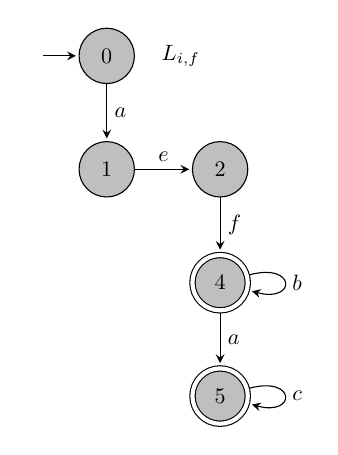
\begin{tikzpicture}
[->,>=stealth, node distance=18mm, auto, initial text=, on grid, shorten >=1pt,
every state/.style={fill=lightgray},
every node/.style={scale=0.8},
accepting/.style={double distance=1.5pt, outer sep=0.75pt+\pgflinewidth}
]
	\node[state, initial]	(0) 					{$0$};
	\node[state]			(1) [below of = 0]		{$1$};
	\node[state]			(2) [right of = 1]		{$2$};
	\node[state, accepting]	(4) [below of = 2]		{$4$};
	\node[state, accepting]	(5) [below of = 4]		{$5$};
	\node[right of = 0] at (-.5,0) {$L_{i,f}$};
	
  	\path
  		(0) edge 				node {$a$} (1)
  		(1) edge 				node {$e$} (2)
  		(2) edge 				node {$f$} (4)
  		(4) edge [loop right]	node {$b$} (4)
  		(4) edge 				node {$a$} (5)
  		(5) edge [loop right]	node {$c$} (5);
\end{tikzpicture}
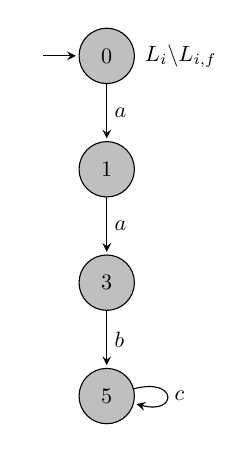
\begin{tikzpicture}
[->,>=stealth, node distance=18mm, auto, initial text=, on grid, shorten >=1pt,
every state/.style={fill=lightgray}, 
every node/.style={scale=0.8},
accepting/.style={double distance=1.5pt, outer sep=0.75pt+\pgflinewidth}
]
	\node[state, initial]	(0) 					{$0$};
	\node[state]			(1) [below of = 0]		{$1$};
% 	\node[state]			(2) [right of = 1]		{$2$};
	\node[state]			(3) [below of = 1]		{$3$};
% 	\node[state]			(4) [right of = 3]		{$4$};
	\node[state]			(5) [below of = 3]		{$5$};
	\node[right of = 0] at (-.5,0) {$L_i\backslash L_{i,f}$};
	
  	\path
  		(0) edge 				node {$a$} (1)
%   		(1) edge 				node {$e$} (2)
  		(1) edge 				node {$a$} (3)
%   		(3) edge 				node {$c$} (4)
  		(3) edge 				node {$b$} (5)
%   		(4) edge [loop right]	node {$b$} (4)
%   		(4) edge 				node {$a$} (5)
  		(5) edge [loop right]	node {$c$} (5);
\end{tikzpicture}
% \tikzset{align at top/.style={baseline=(current bounding box.north)}}
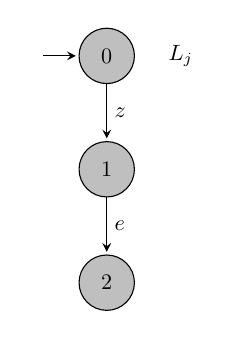
\begin{tikzpicture}
[->,>=stealth, node distance=18mm, auto, initial text=, on grid, shorten >=1pt,
every state/.style={fill=lightgray},
every node/.style={scale=0.8}, 
accepting/.style={double distance=1.5pt, outer sep=0.75pt+\pgflinewidth}
]
	\node[state, initial]	(0) 			{$0$};
	\node[state]			(1) [below of = 0]		{$1$};
	\node[state]			(2) [below of = 1]		{$2$};
	\node[right of = 0] at (-.5,0) {$L_j$};
	
  	\path
  		(0) edge 				node {$z$} (1)
  		(1) edge 				node {$e$} (2);
\end{tikzpicture}
\caption{Automata representing faulty $L_{i,f}$ and
non-faulty $L_i \backslash L_{i,f}$ languages of one module, and the language
$L_j$ of a second module. Given $\Sigma_o = \{b, c, z\}$ the language $L_i
\parallel L_j$ is not diagnosable.}
\label{fig_changed_observation}
\end{figure}

\begin{example} Consider one module the language $L_i$ as depicted in
Figure \ref{fig_automaton_F-NF} and another module with a language $L_j$ as
depicted in Figure \ref{fig_changed_observation}. At the last figure the
only strings of $L_i$ which form indeterminate cycles are presented, assuming that 
$\Sigma_o = \{b, c, z\}$. The language $L_i$ is not diagnosable since it has
indeterminate cycle $\{bc^*\}$. If both $L_i$ and $L_j$ are composed
(depicted in Figure \ref{fig_example_parallel}), then, as it
stated in the Conjecture \ref{cnj_changed_observation}, the all string in
$L_{i,f}$ change their observation.
However, whenever the event $z$ is observed any string of $L_i\backslash
L_{i,f}$ can be executed in the language $L_i \parallel L_j$.
Thus, the composed system is not diagnosable either.
\end{example}

The reason the observation changing does not affect diagnosability in the
above example is that the non-faulty language $L_i\backslash L_{i,f}$ with its 
strings which form indeterminate cycle are included in the inverse projection of
$M(L_j)$, i.e.
$
L_i\backslash L_{i,f} \subseteq P_i^{-1}(M(L_j)).
$
Henceforth, we need to prohibit the execution of the observable event $z$
in $L_j$ until some traces in $L_i$ are executed. The only way to do it is to
make all the prefixes of the language $L'_j$ (defined in Conjecture
\ref{cnj_changed_observation}) having common events, as it is shown in the
following example.

\begin{figure}[t]
\centering
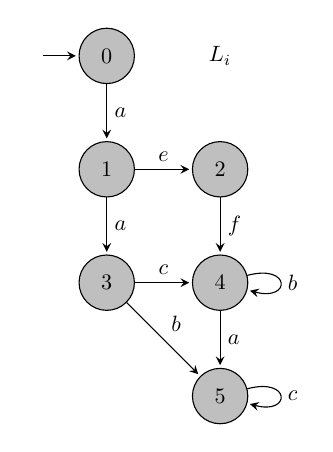
\begin{tikzpicture} 
[->,>=stealth, node distance=18mm, auto, initial text=, on grid,
shorten >=1pt, every state/.style={fill=lightgray}, 
every node/.style={scale=0.8}, 
accepting/.style={double distance=1.5pt, outer sep=0.75pt+\pgflinewidth}] 
	\node[state, initial]	(0) 					{$0$};
	\node[state]			(1) [below of = 0]		{$1$};
	\node[state]			(2) [right of = 1]		{$2$};
	\node[state]			(3) [below of = 1]		{$3$};
	\node[state]			(4) [right of = 3]		{$4$};
	\node[state]			(5) [below of = 4]		{$5$};
	\node[right of = 0] at (0,0) {$L_i$};
		
  	\path
  		(0) edge 				node {$a$} (1)
  		(1) edge 				node {$e$} (2)
  		(1) edge 				node {$a$} (3)
  		(2) edge 				node {$f$} (4)
  		(3) edge 				node {$c$} (4)
  		(3) edge 				node {$b$} (5)
  		(4) edge [loop right]	node {$b$} (4)
  		(4) edge 				node {$a$} (5)
  		(5) edge [loop right]	node {$c$} (5);
\end{tikzpicture}
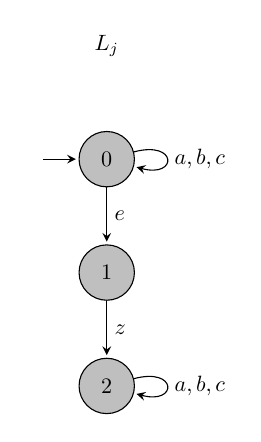
\begin{tikzpicture}
[->,>=stealth, node distance=18mm, auto, initial text=, on grid, shorten >=1pt,
every state/.style={fill=lightgray},
every node/.style={scale=0.8}, 
accepting/.style={double distance=1.5pt, outer sep=0.75pt+\pgflinewidth}
]
	\node[state, initial]	(0) 					{$0$};
	\node[state]			(1) [below of = 0]		{$1$};
	\node[state]			(2) [below of = 1]		{$2$};
	\node[above of = 0] at (0,0) {$L_j$};
	
  	\path
  		(0) edge [loop right]	node {$a, b, c$} (0)
  		(0) edge 				node {$e$} (1)
  		(1) edge 				node {$z$} (2)
  		(2) edge [loop right]	node {$a, b, c$} (2);
\end{tikzpicture}
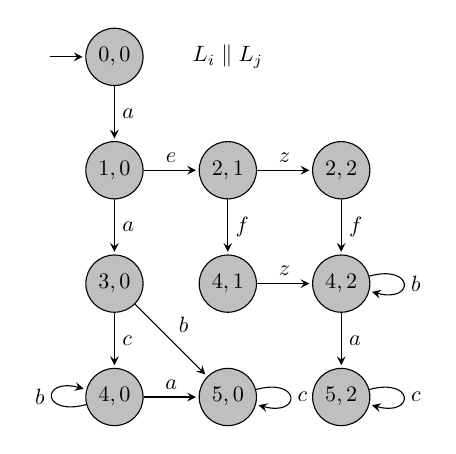
\begin{tikzpicture}
[->,>=stealth, node distance=18mm, auto, initial text=, on grid, shorten >=1pt,
every state/.style={fill=lightgray},
every node/.style={scale=0.8}, 
accepting/.style={double distance=1.5pt, outer sep=0.75pt+\pgflinewidth}
]
	\node[state, initial]	(00) 					{$0,0$};
	\node[state]			(10) [below of = 00]	{$1,0$};
	\node[state]			(21) [right of = 10]	{$2,1$};
	\node[state]			(22) [right of = 21]	{$2,2$};
	\node[state]			(41) [below of = 21]	{$4,1$};
	\node[state]			(42) [right of = 41]	{$4,2$};
	\node[state]			(52) [below of = 42]	{$5,2$};
	\node[state]			(30) [below of = 10]	{$3,0$};
	\node[state]			(40) [below of = 30]	{$4,0$};
	\node[state]			(50) [below of = 41]	{$5,0$};
 	\node[right of = 00] at (0,0) {$L_i \parallel L_j$};
	
   	\path
   		(00) edge 				node {$a$} (10)
   		(10) edge 				node {$e$} (21)
   		(10) edge 				node {$a$} (30)
   		(30) edge 				node {$c$} (40)
   		(30) edge 				node {$b$} (50)
   		(40) edge 				node {$a$} (50)
   		(21) edge 				node {$z$} (22)
   		(21) edge 				node {$f$} (41)
   		(22) edge 				node {$f$} (42)
   		(41) edge 				node {$z$} (42)
   		(50) edge [loop right]	node {$c$} (50)
   		(40) edge [loop left]	node {$b$} (40)
   		(42) edge [loop right]	node {$b$} (42)
   		(42) edge 				node {$a$} (52)
   		(52) edge [loop right]	node {$c$} (52);
\end{tikzpicture}
\caption{Automata representing the language $L_i$ and the language $L_j$ which
makes the language $L_i \parallel L_j$ diagnosable, given 
$\Sigma_o = \{b, c, z\}$}
\label{fig_changed_observation2}
\end{figure}

\begin{example} In the Figure \ref{fig_changed_observation2} the language $L_i$
has indistinguishable strings which form indeterminate cycle. The language
$L_j$ satisfies the condition of the Conjecture \ref{cnj_changed_observation}
since all the continuation of strings starting from the state $2$ have the
observable event $z$ in the prefixes. Moreover, event $z$ does not occur until 
event $e$ is executed. It can be checked, that the parallel composition of the
languages $L_i$ and $L_j$ breaks indeterminate cycle, and the resulting
language is diagnosable.

Note: The non-blocking assumption is violated in this particular example (for
instance, 
$\{a^*\} \in L_j$ but $\{a^*\} \not \in P^{-1}_j(L_i \parallel L_j)$).
\end{example}

More formally, we require a set of strings 
$\{\Sigma_j \sigma't\sigma''\} \subseteq L_j \mid \sigma', 
\sigma'' \in \Sigma_i \cap \Sigma_j$ be observable: $M(t) \neq \emptyset$
(this projection is equal to one define in \ref{cnj_changed_observation}),
and all the common events be either in faulty or non-faulty sub-language of
$L_i$, i.e 
$$
	P_{i,j}^{-1}(L_j) \cap L_{i,f} = L_{i,f} \textrm{ or } 
	P_{i,j}^{-1}(L_j) \cap L_i\backslash \overline{L_{i,f}} 
	= L_i\backslash \overline{L_{i,f}}.
$$
The above condition is sufficient to make the system diagnosable. In other cases
the compositional process is required.

In order to check the above requirements a verification procedure might be as
follows (note, the complexity is linear):
\begin{enumerate}
  \item Mark the language $L_{i,f}$ by the automaton depicted in Figure
  \ref{fig_marking_two_common}, left;
  \item Mark the language $L_i\backslash \overline{L_{i,f}}$ the same way;
  \item Check if only one marked language is not empty, and all strings of that
  language reach the marked states. Continue if it is true, otherwise stop the
  procedure;
  \item Mark the language $L_j$ by the automaton depicted in Figure
  \ref{fig_marking_two_common}, right;
  \item If the marked language is not empty then declare the system is
  diagnosable, otherwise declare the system is not diagnosable.
\end{enumerate}

\begin{figure}[t]
\centering
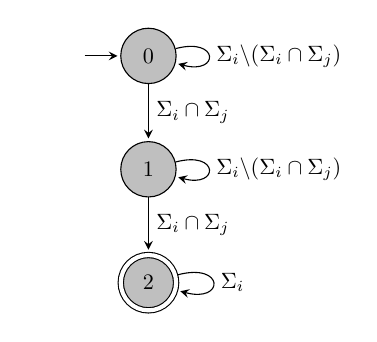
\begin{tikzpicture}
[->,>=stealth, node distance=18mm, auto, initial text=, on grid, shorten >=1pt,
every state/.style={fill=lightgray},
every node/.style={scale=0.8}, 
accepting/.style={double distance=1.5pt, outer sep=0.75pt+\pgflinewidth}
]
	\node[state, initial]	(0) 				{$0$};
	\node[state]			(1) [below of = 0]	{$1$};
	\node[state, accepting]	(2) [below of = 1]	{$2$};
	\node[left of = 0] at (0,0) {$$};

  	\path
  		(0) edge [loop right]
  			node {$\Sigma_i \backslash (\Sigma_i \cap \Sigma_j)$} (0) 
  		(0) edge
  			node {$\Sigma_i \cap \Sigma_j$} (1) 
  		(1) edge [loop right]
  			node {$\Sigma_i \backslash (\Sigma_i \cap \Sigma_j)$} (1) 
  		(1) edge
  			node {$\Sigma_i \cap \Sigma_j$} (2) 
  		(2) edge [loop right]
  			node {$\Sigma_i $} (2); 
\end{tikzpicture}
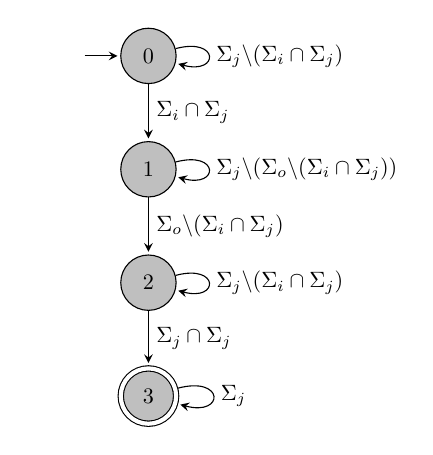
\begin{tikzpicture}
[->,>=stealth, node distance=18mm, auto, initial text=, on grid, shorten >=1pt,
every state/.style={fill=lightgray},
every node/.style={scale=0.8}, 
accepting/.style={double distance=1.5pt, outer sep=0.75pt+\pgflinewidth}
]
	\node[state, initial]	(0) 				{$0$};
	\node[state]			(1) [below of = 0]	{$1$};
	\node[state]			(2) [below of = 1]	{$2$};
	\node[state, accepting]	(3) [below of = 2]	{$3$};
	\node[left of = 0] at (0,0) {$$};

  	\path
  		(0) edge [loop right]
  			node {$\Sigma_j \backslash (\Sigma_i \cap \Sigma_j)$} (0) 
  		(0) edge
  			node {$\Sigma_i \cap \Sigma_j$} (1) 
  		(1) edge [loop right]
  			node {$\Sigma_j \backslash (\Sigma_o \backslash (\Sigma_i \cap	\Sigma_j))$} (1) 
  		(1) edge
  			node {$\Sigma_o \backslash (\Sigma_i \cap	\Sigma_j)$} (2) 
  		(2) edge [loop right]
  			node {$\Sigma_j \backslash (\Sigma_i \cap \Sigma_j)$} (2) 
  		(2) edge
  			node {$\Sigma_j \cap \Sigma_j$} (3) 
  		(3) edge [loop right]
  			node {$\Sigma_j $} (3); 
\end{tikzpicture}
\caption{Automata for marking the languages $L_i$ and $L_j$}
\label{fig_marking_two_common}
\end{figure}

We proceed by establishing a necessary condition for diagnosability by an
adjacent module. The non-blocking assumption is relaxed in the following.
Firstly we define a \emph{potentially non-blocking} string for the language of
an adjacent module:

\begin{definition} A string $s \in L_j$ is potentially non-blocking with respect
to any string from $L_i$ if there is no a string with more then two common events
in it, and the common event is in the strongly connected component, i.e:
$$
\begin{array}{l}
	(\forall \sigma, \sigma' \in \Sigma_i \cap \Sigma_j \mid \sigma \neq
	\sigma') 
	[\not \exists ~\Sigma_j \sigma \Sigma_j \sigma' \in \overline{s}]
	\textrm{ and} \\
	(\forall ~\Sigma_j \sigma \in \overline{s}) 
	[\exists \Sigma_j \sigma t \in \overline{s} \mid \Sigma_j \sigma \in \overline{t}]
	
\end{array}
$$
\end{definition}
Consequently, a \emph{potentially blocking} string is a string which has more
then one common events in it, or the common event is not in a strongly connected
component. It worth noting that this definition has no assumptions about the
strings of the language $L_i$. However, there are conditions of non-blocking
when the structure of both languages is known. For instance, the case when 
languages have strings with one common event and this event is in a strongly
connected component or not, equally for both languages. These cases reflected in
the two conjectures below (skip them to proceed to a more general condition).

\begin{conjecture}[SCC with one common event] If an adjacent module has a
common event only in its strongly connected component (SCC), and that event is
common only to events in the indeterminate cycle (which is a SCC as well), then
the composition does not change the diagnosability property.
\end{conjecture} 

The proof of the above conjecture seems trivial, since any prefix of the
adjacent module's SCC before the common event forms an interleaving with the
language of non-diagnosable module. And the SCC itself is projected to the only
state with respect to the common event, no matter how many observable
events the SCC has.

\begin{conjecture}[SCC with many common events] If an adjacent module has 
common events only in its strongly connected component (SCC), and those events
are common only to events in the indeterminate cycle (which is a SCC as well),
then the composition does not change the diagnosability property.
\end{conjecture}

In the above conjecture if the both SCC have the same projection with respect to
the common events then the indeterminate cycle is not changing. Otherwise it
might be or not changed due to blocking. Nevertheless, the observable
projection of the adjacent SCC changes an observable projection of
the indeterminate cycle equally for both faulty and non-faulty strings.

A weakest, most general condition for changing diagnosability by an
adjacent module is the next:

\begin{conjecture}[Necessary condition for changing diagnosability] Given two
languages $L_i$ and $L_j$, and the a faulty behaviour is defined only for $L_i$.
Diagnosability property of $L_i$ can be changed by the parallel composition $L_i
\parallel L_j$ only if the language $L_j$ has a potentially blocking string with
respect to another language.
% \begin{equation}
% L_{j,s}^{>1} \neq \emptyset
% \end{equation}
\end{conjecture}
% In the above, $L_{j,s}^{>1} \neq \emptyset \Rightarrow L_{i,s}^{1} \neq \emptyset$ 


% $$
% \begin{array}{l}
% 	P_{i,j}^{-1}(L_{i,f}) \cap P_{i,j}^{-1}(L_i \backslash L_{i,f})
% \end{array}
% $$



% From the above we can see that the assumption of Contant that the common events
% are observable, actually does not affect the observability property.

%%%%%%%%%%%%%%%%%%%%%%%%%%%%%%%%%%%%%%%%%%%%%%%%%%%%%%%%%%%%%%%%%%%%%%%%%%%%%%%
% \section{todo:}
% \begin{enumerate}
%   \item Who defines the models of the components? 
%   \item What exactly makes modular diagnoses different from each other?
%   \item Check for approaches where the number of diagnosers varies.
% \end{enumerate}
\begin{figure}[ht]
\centering
	\includegraphics[height=95mm]{parallel.jpg}
	\caption{The result of the parallel composition of the languages depicted in
	Figure \ref{fig_changed_observation} (Looks ugly? Thanks DESUMA)}
	\label{fig_example_parallel}
\end{figure}

%%%%%%%%%%%%%%%%%%%%%%%%%%%%%%%%%%%%%%%%%%%%%%%%%%%%%%%%%%%%%%%%%%%%%%%%%%%%%%%
\section{Conclusion}
\label{sec:Conclusion}

%\addtolength{\textheight}{-16.7cm}   % This command serves to balance the
% column lengths
                                  % on the last page of the document manually. It shortens
                                  % the textheight of the last page by a suitable amount.
                                  % This command does not take effect until the next page
                                  % so it should come on the page before the last. Make
                                  % sure that you do not shorten the textheight too much.

\bibliographystyle{IEEEtran}
\bibliography{References}

\newpage
\section{Excluded from the paper but might be useful}
\begin{figure}[ht]
\centering
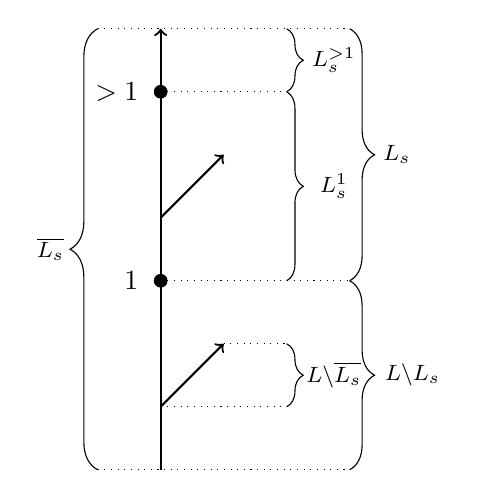
\begin{tikzpicture}[scale=.8]
\draw [thick] [->](2,1)--(2,8);
\draw [thick] [->](2,2)--(3,3);
\draw [thick] [->](2,5)--(3,6);
% Events
\draw [fill] (2,4) circle [radius=0.1];
\node [left] at (1.8,4) {$1$};
\draw [fill] (2,7) circle [radius=0.1];
\node [left] at (1.8,7) {$>1$};
% Braces
\draw [decorate,decoration={brace,amplitude=10pt}]
 	(1,1)--(1,8) node [midway,xshift=-0.6cm] {\footnotesize $\overline{L_s}$};
\draw [decorate,decoration={brace,amplitude=6pt}]
 	(4,8)--(4,7) node [midway,xshift=0.6cm] {\footnotesize $L^{>1}_s$};
\draw [decorate,decoration={brace,amplitude=6pt}]
 	(4,7)--(4,4) node [midway,xshift=0.6cm] {\footnotesize $L^{1}_s$};
\draw [decorate,decoration={brace,amplitude=9pt}]
 	(5,8)--(5,4) node [midway,xshift=0.6cm] {\footnotesize $L_s$};
\draw [decorate,decoration={brace,amplitude=6pt}]
 	(4,3)--(4,2) node [midway,xshift=0.6cm] {\footnotesize $L \backslash
 	\overline{L_s}$};
\draw [decorate,decoration={brace,amplitude=9pt}]
 	(5,4)--(5,1) node [midway,xshift=0.8cm] {\footnotesize $L \backslash L_s$};
%Dashed lines
\draw [dotted] (1,8)--(5,8);
\draw [dotted] (2,7)--(4,7);
\draw [dotted] (2,4)--(5,4);
\draw [dotted] (3,3)--(4,3);
\draw [dotted] (2,2)--(4,2);
\draw [dotted] (1,1)--(5,1);
\end{tikzpicture}
\caption{Structural schema of the definition of the synchronized language
$L_s$ over a language $L$}
\label{fig_partitioning_synch}
\end{figure}

For the sake of clarity we introduce a structural schema of the
synchronized language defined by \ref{eq_synchronized_language} in Section
\ref{sec:definitions}. It is depicted in Figure \ref{fig_partitioning_synch}.
(In the figure the language $L_s$ is equal to $L'$ in \ref{sec:definitions}).

\end{document}
